%%%%%%%%%%%%%%%%%%%%%%%%%%%%%%%%%%%%%%%%%%%%%%%%%%%%%%%%%%%%%%%%
% %
% Seth Cram %
% ECE351 Section 53 %
% Lab 10 %
% Due 04/05/2022 %
% Any other necessary information needed to navigate the file %
%
%
% %
%%%%%%%%%%%%%%%%%%%%%%%%%%%%%%%%%%%%%%%%%%%%%%%%%%%%%%%%%%%%%%%%
%%%%%%%%%%%%%%%%%%%%%%%%%%%%%%%%%%%%%%%%%%%
%%% DOCUMENT PREAMBLE %%%
\documentclass[12pt]{report}
\usepackage[english]{babel}
%\usepackage{natbib}
\usepackage{url}
\usepackage[utf8x]{inputenc}
\usepackage{amsmath}
\usepackage{graphicx}
\graphicspath{{images/}}
\usepackage{parskip}
\usepackage{fancyhdr}
\usepackage{vmargin}
\usepackage{listings}
\usepackage{hyperref}
\usepackage{xcolor}
\usepackage{verbatim}
\usepackage{listings}

\definecolor{codegreen}{rgb}{0,0.6,0}
\definecolor{codegray}{rgb}{0.5,0.5,0.5}
\definecolor{codeblue}{rgb}{0,0,0.95}
\definecolor{backcolour}{rgb}{0.95,0.95,0.92}

\begin{comment} %have to use verbatim package for this

\section{Personal Notes}
            


\end{comment}

\lstdefinestyle{mystyle}{
    backgroundcolor=\color{backcolour},   
    commentstyle=\color{codegreen},
    keywordstyle=\color{codeblue},
    numberstyle=\tiny\color{codegray},
    stringstyle=\color{codegreen},
    basicstyle=\ttfamily\footnotesize,
    breakatwhitespace=false,         
    breaklines=true,                 
    captionpos=b,                    
    keepspaces=true,                 
    numbers=left,                    
    numbersep=5pt,                  
    showspaces=false,                
    showstringspaces=false,
    showtabs=false,                  
    tabsize=2
}
 
\lstset{style=mystyle}

\setmarginsrb{3 cm}{2.5 cm}{3 cm}{2.5 cm}{1 cm}{1.5 cm}{1 cm}{1.5 cm}

\title{Lab 10}		%TITLE						
% Title
\author{ Seth Cram}						
% Author
\date{04/05/2022}
% Date

\makeatletter
\let\thetitle\@title
\let\theauthor\@author
\let\thedate\@date
\makeatother

\pagestyle{fancy}
\fancyhf{}
\rhead{\theauthor}
\lhead{\thetitle}
\cfoot{\thepage}
%%%%%%%%%%%%%%%%%%%%%%%%%%%%%%%%%%%%%%%%%%%%
\begin{document}

%%%%%%%%%%%%%%%%%%%%%%%%%%%%%%%%%%%%%%%%%%%%%%%%%%%%%%%%%%%%%%%%%%%%%%%%%%%%%%%%%%%%%%%%%

\begin{titlepage}
	\centering
    \vspace*{0.5 cm}
   % \includegraphics[scale = 0.075]{bsulogo.png}\\[1.0 cm]	% University Logo
\begin{center}    \textsc{\Large   ECE 351 - 53 }\\[2.0 cm]	\end{center}% University Name
	\textsc{\Large Frequency Response }\\[.5 cm]				% Course Code
	\rule{\linewidth}{0.2 mm} \\[0.4 cm]
	{ \huge \bfseries \thetitle}\\
	\rule{\linewidth}{0.2 mm} \\[1.5 cm]
	
	\begin{minipage}{0.4\textwidth}
		\begin{flushleft} \large
		%	\emph{Submitted To:}\\
		%	Name\\
          % Affiliation\\
           %contact info\\
			\end{flushleft}
			\end{minipage}~
			\begin{minipage}{0.4\textwidth}
            
			\begin{flushright} \large
			\emph{Submitted By :} \\
			Seth Cram  
		\end{flushright}
           
	\end{minipage}\\[2 cm]
	
\end{titlepage}

%%%%%%%%%%%%%%%%%%%%%%%%%%%%%%%%%%%%%%%%%%%%%%%%%%%%%%%%%%%%%%%%%%%%%%%%%%%%%%%%%%%%%%%%%

\tableofcontents
\pagebreak

%%%%%%%%%%%%%%%%%%%%%%%%%%%%%%%%%%%%%%%%%%%%%%%%%%%%%%%%%%%%%%%%%%%%%%%%%%%%%%%%%%%%%%%%%
\renewcommand{\thesection}{\arabic{section}}

\section{Introduction}

The goal of lab 10 is to become familiar with frequency response tools and Bode plots using Python in the Spyder IDE.

\section{Equations}
    \begin{equation}
        H(s) = \frac{\frac{1}{RC}s}{s^2+\frac{1}{RC}s+\frac{1}{LC}} 
    \end{equation}
    \begin{equation}
        |H(j\omega)| = \frac{(w/(R*C))}{\sqrt(w^4 + ((1/(R*C))^2 - 2/(L*C))*(w^2) + (1/(L*C))^2)}  
    \end{equation}
    \begin{equation}
        phase \; of \; H(j\omega) = \pi/2 - arctan(\frac{(w/(R*C))}{(-1*(w^2)+(1/(L*C))))} 
    \end{equation}
    \begin{equation}
        x(t) = cos(2\pi 100t) + cos(2\pi 3024t) + sin(2\pi 50000t)
    \end{equation}
    
\section{Methodology}

%This section will describe how you went about solving the lab. Make sure you go into detail about any method you used. %Include coding samples here if necessary. This is also where you would include necessary derivations. An example of %inserting code into the report is given. Do not go overboard on inserting code into your report, only use whats %absolutely necessary to illustrate your point.

    \paragraph{} First, I redid the prelab correctly. Then, I used that expression to make the bode plot. First, I had to convert magnitude to dB and phase to degrees. These were simple conversions. Making the plot, I had to make the step size relatively large or else the calculations would take much longer later on. I used the logarithmic plotting function on the x-axis to achieve an appropriate bode plot. I had to adjust the second half of the phase down 180 degrees to get a nice looking plot. 
    
    \paragraph{} Second, I used the scipy bode plot function to plot magnitude and phase response of the transfer function. I checked and made sure both plots matched before moving on. 
    
    \paragraph{} Third, to get a frequency response, I imported the control package and used its transfer and bode functions. Interestingly enough, the bode function plotted the function for us, given the correct settings. 
    
    \paragraph{} Fourth, I plotted the give x(t) with a sampling frequency equivalent to its largest $w_0$ term. Doing so gave me a clean plot on the tiny length of time I plotted over. 
    
    \paragraph{} To pass the input signal through the transfer function, I needed to convert said function into its z-domain equivalent. After doing so, I passed the input signal through the filter, both steps using separate scipy.signal functions. Finally, I plotted the output signal $y(t)$ over the same time period as the previous graph for comparison sake. 
    
\section{Results}

%This section will go over the results of the lab. Use this area to describe %if the lab worked as expected or if the results are unexpected or different %from your hand calculations or intuition. Part of being a good engineer is %gaining intuition about these problems and being able to understand quickly %if something is wrong. Use code, plots, tables, and figures as necessary. %Make sure to cite all other works used and note them in the bibliography. A %sample entry is in this document.
    
    \paragraph{} Initially, given the original transfer function, I expected a two pole transfer function. So, I thought it'd go through a 180 degree change in its phase graph.    
    
    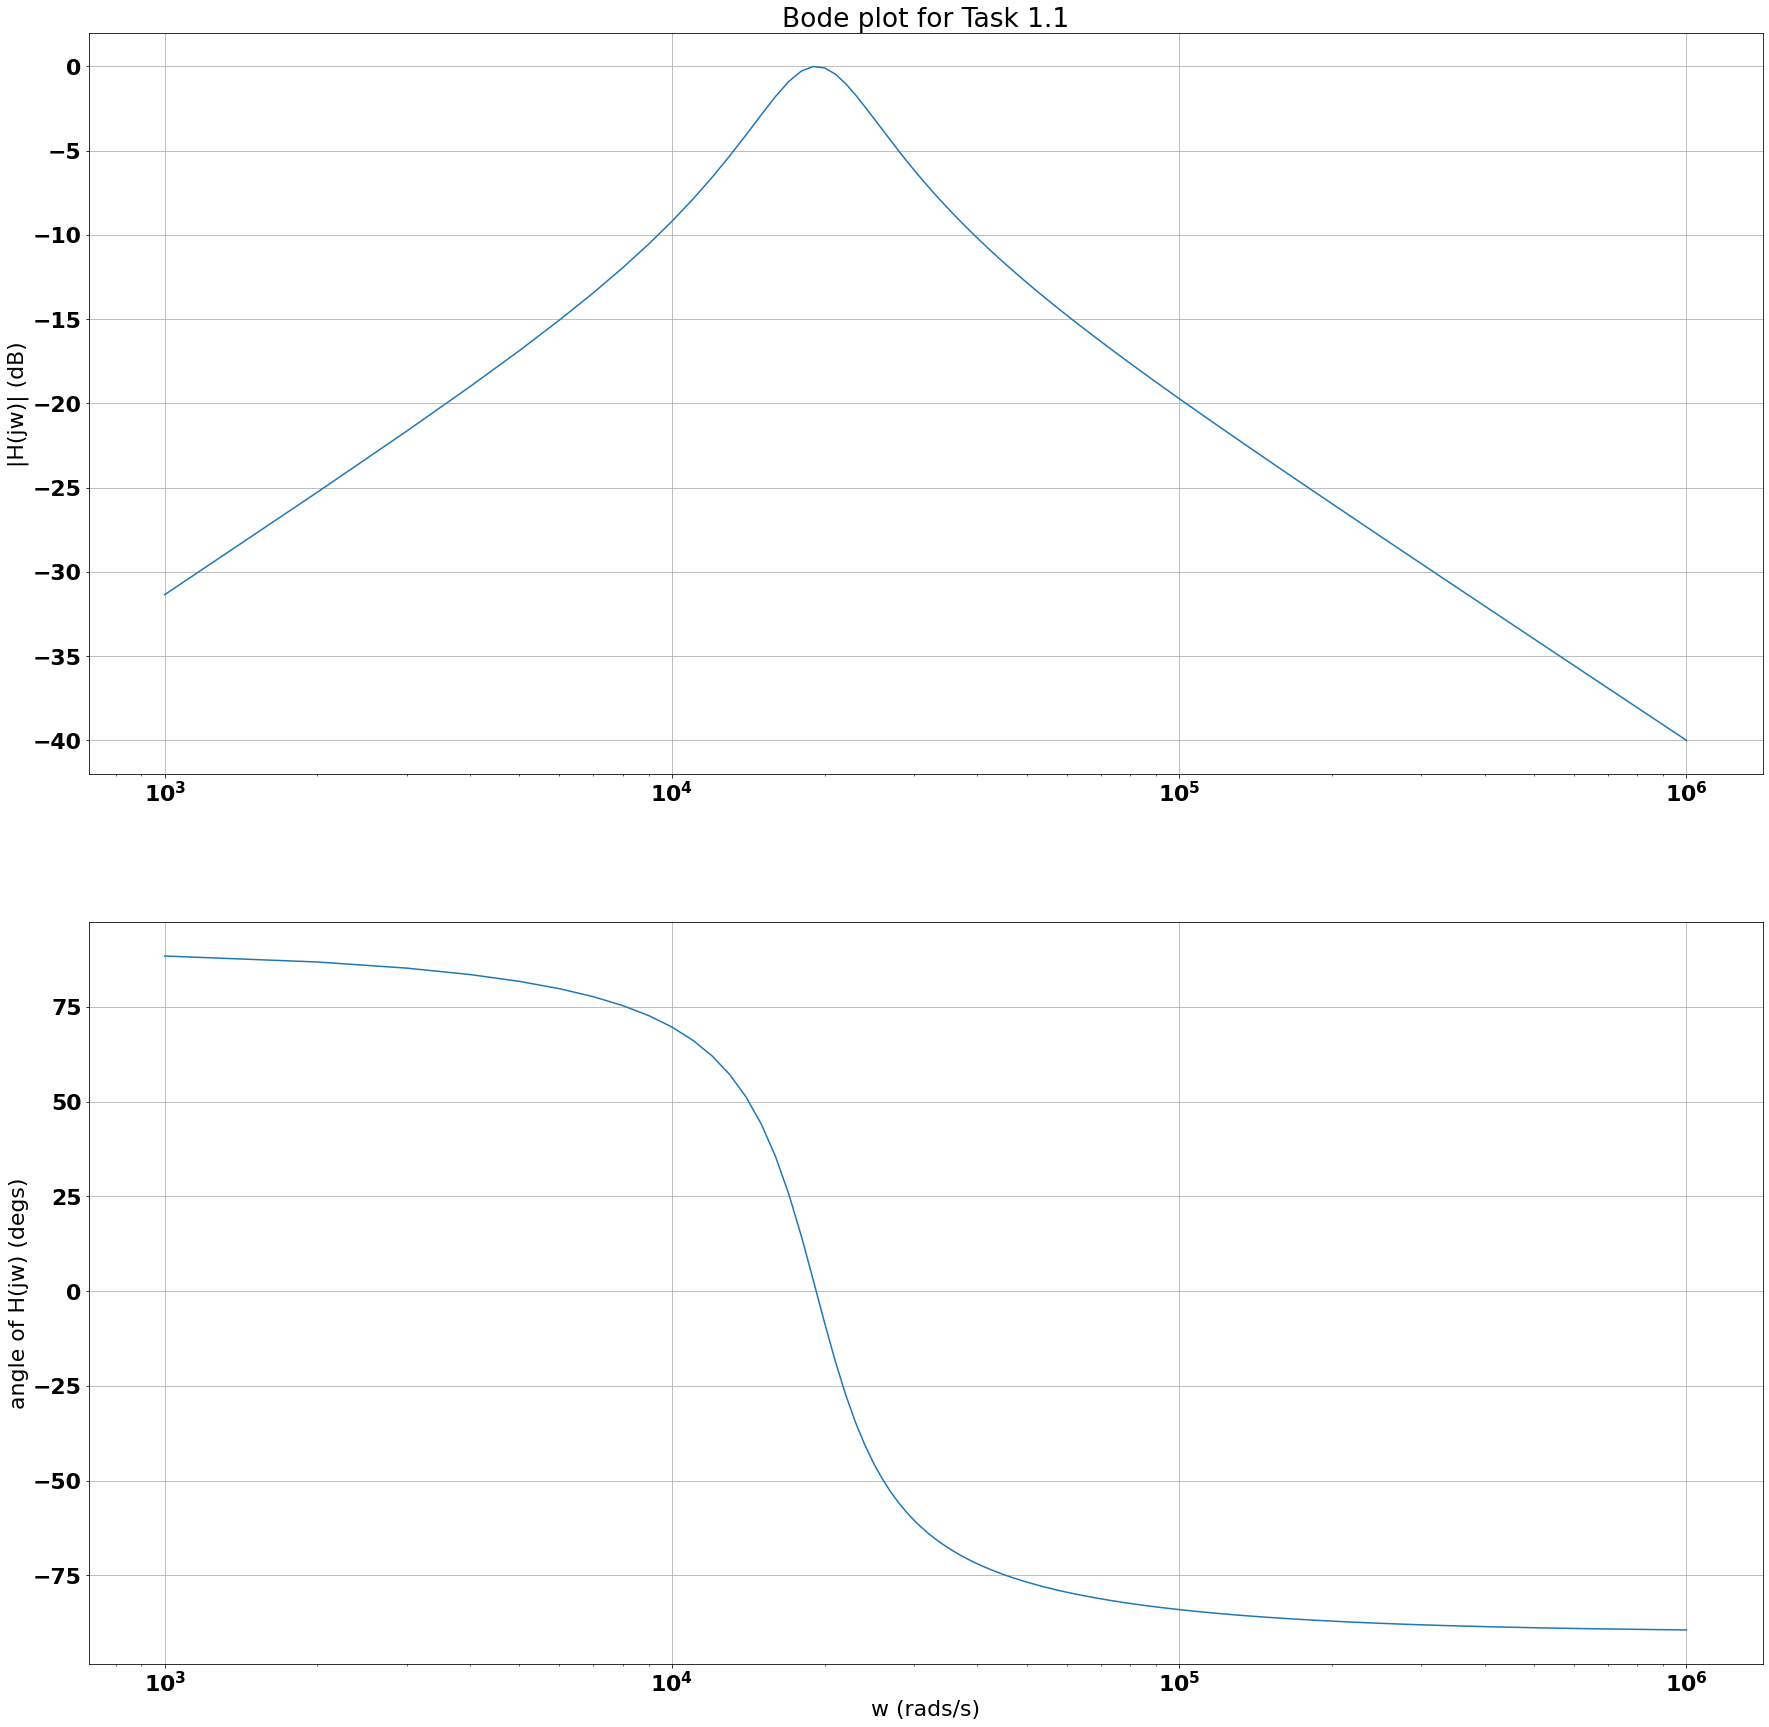
\includegraphics[scale=0.25]{Figure 2022-03-29 221910 (0).png}
    
    \paragraph{} As seen above, my expectation was proven true since it starts at 90 degrees and ends at -90 degrees.  

    \paragraph{} I expected the library function to output the same function as seen previously, without the extra need of shifting 180 degrees on the second half.   
    
    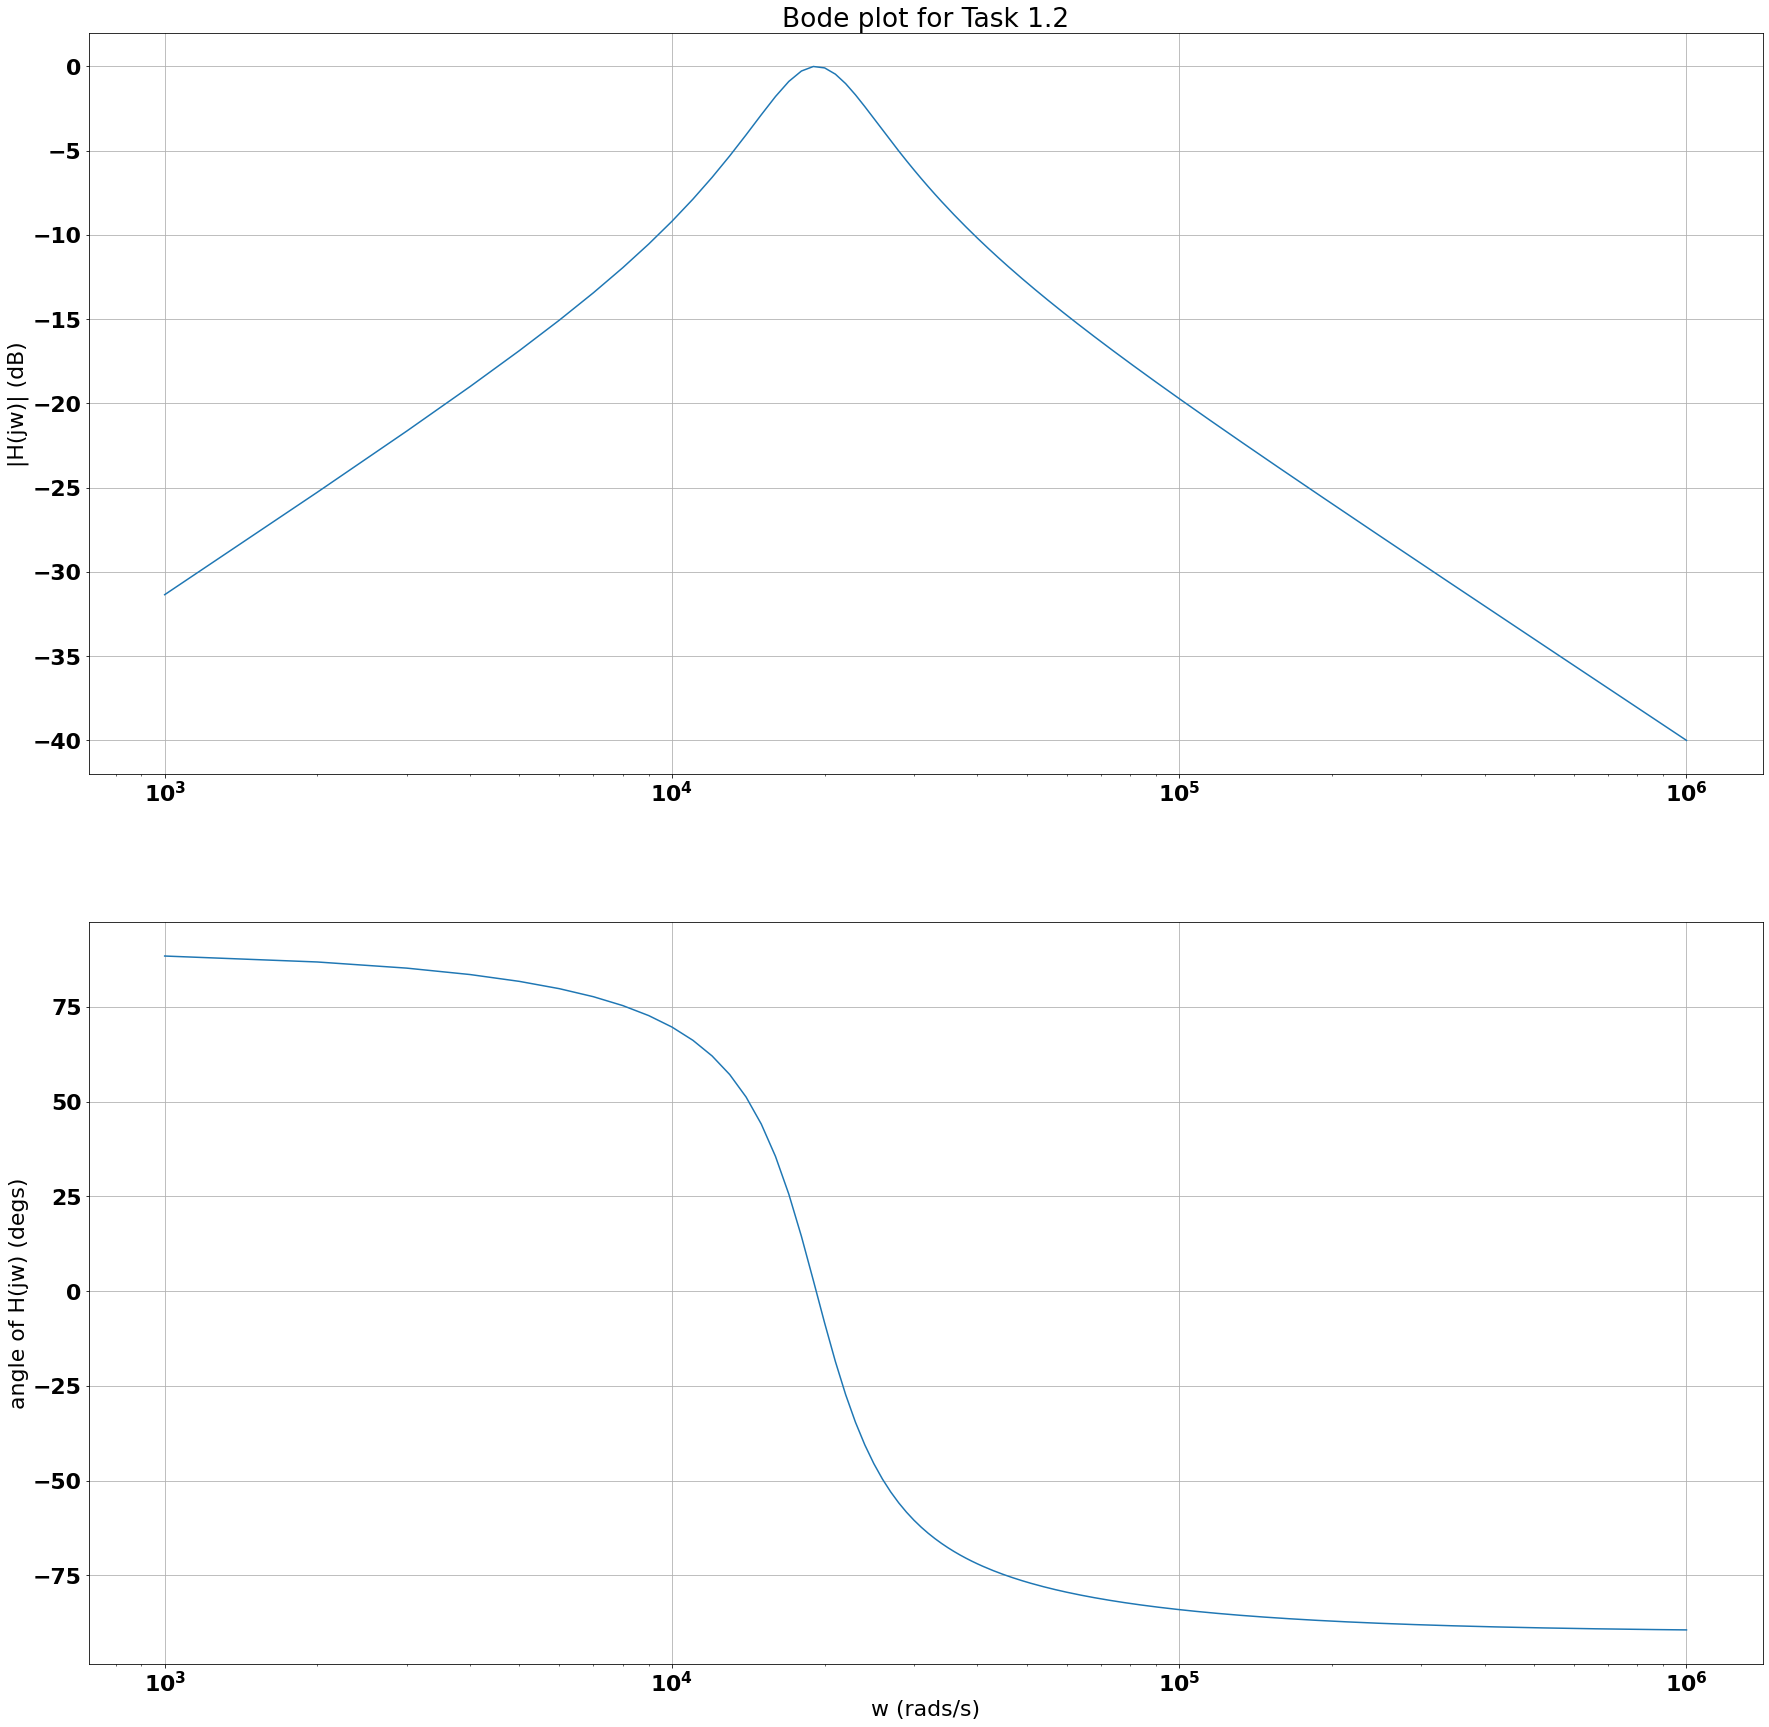
\includegraphics[scale=0.25]{Figure 2022-03-29 221910 (1).png}
    
    \paragraph{} As seen above, my expectations once again proved true. The plot was directly from the library function with no extra altering. 

    \paragraph{} I expected some major differences from my previous two graphs since I'd now be graphing wrt Hz instead of rad/s.    
    
    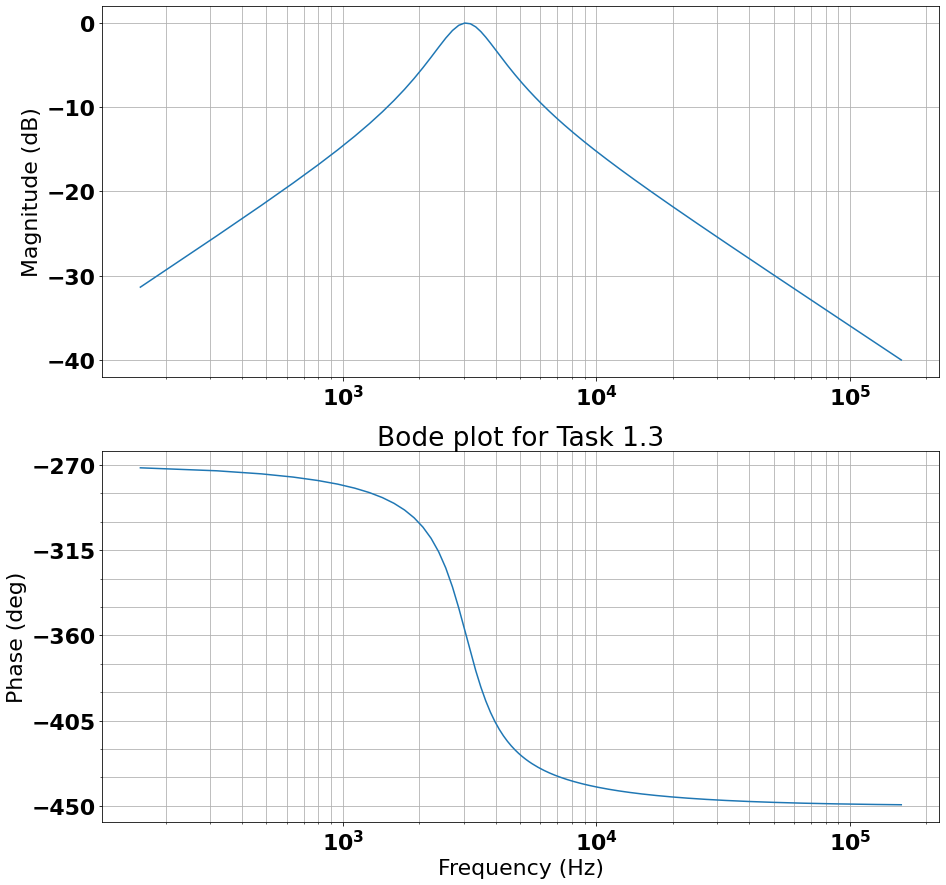
\includegraphics[scale=0.25]{Figure 2022-03-29 221910 (2).png}
    
    \paragraph{} As seen above, it's kind of hard to tell since the phase's y-axis is shifted down an entire -360 degrees, but this graph is almost the exact same as the previous two. So, my expectations were proven wrong this time. 

    \paragraph{} Since x(t) held various sinusoidal terms, I expected a great deal of attenuation and signal variation.    
    
    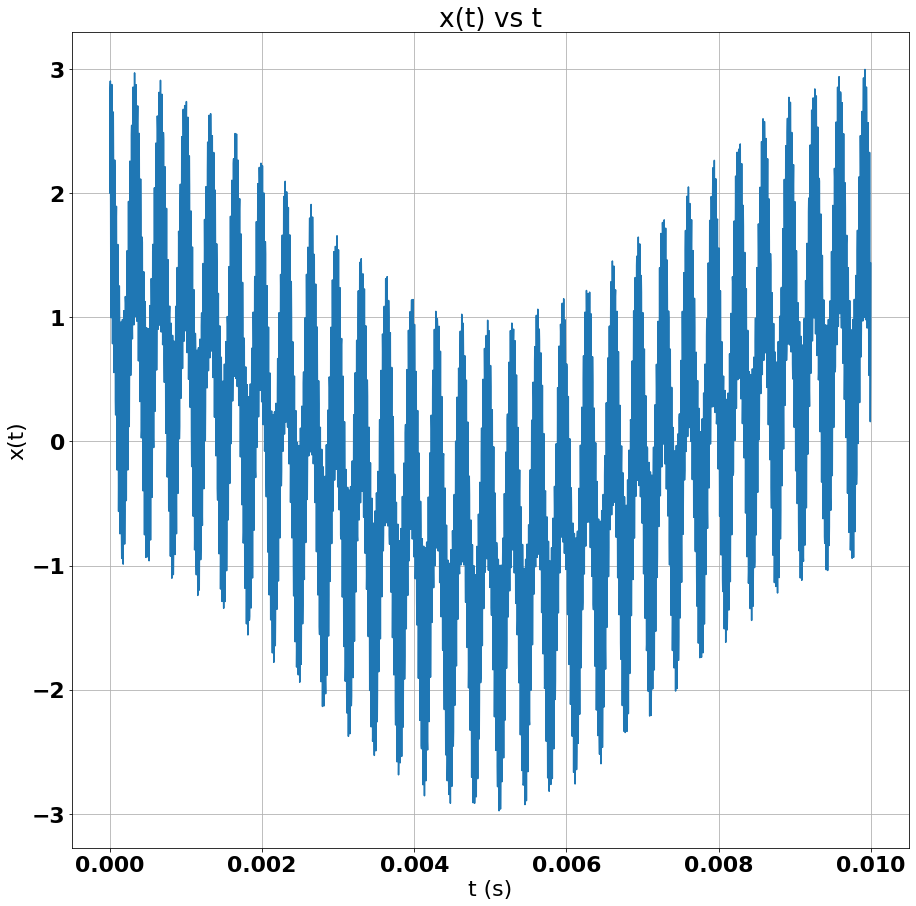
\includegraphics[scale=0.25]{Figure 2022-03-29 221910 (3).png}
    
    \paragraph{} As seen above, my expectations held truer than I originally believed. I received a great deal of attenuation, along with a u shape. 
    
    \paragraph{} After transforming the input function by putting it through the filter, I expected less attenuating. The bode plots showed that the transfer function should attenuate and change the phase of both the first and last sinusoidal terms in x(t) because of their $w_0$'s. 
    
    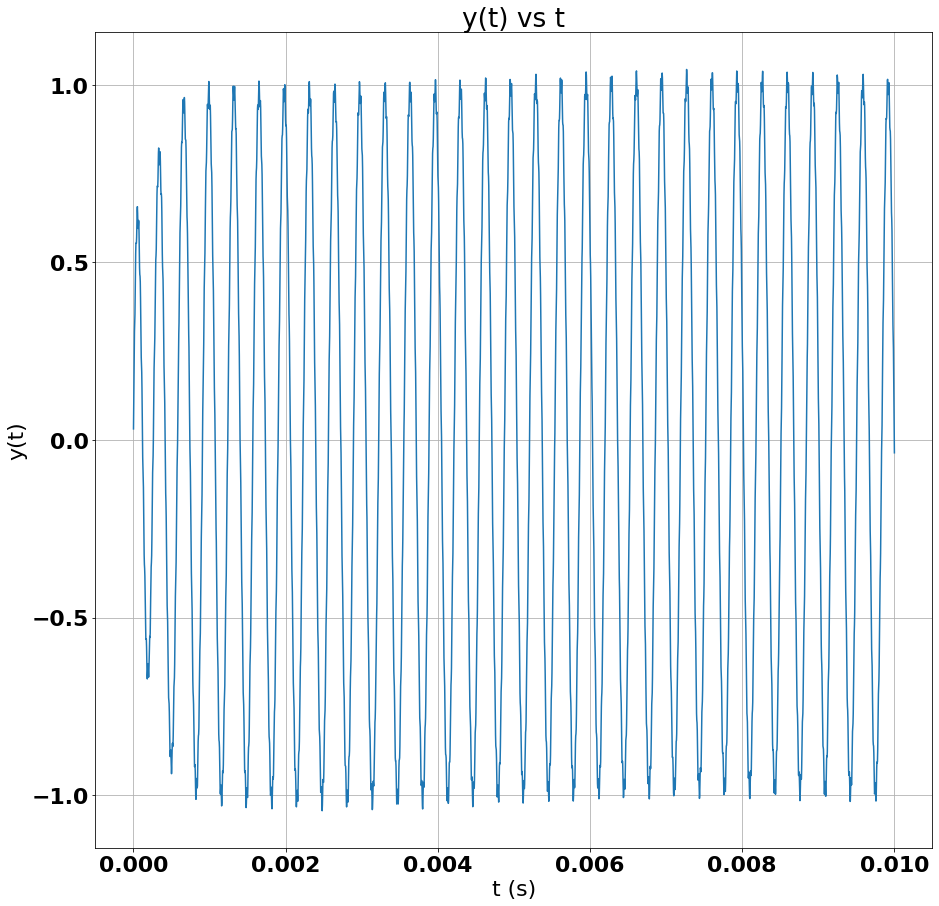
\includegraphics[scale=0.25]{Figure 2022-03-29 221910 (4).png}
    
    \paragraph{} My expectations proved somewhat true. Although there was less overall attenuation concerning magnitude, the shape changed to a flat line, correcting the u shape of the first graph. 

\section{Error Analysis}

%This section will discuss error analysis of the experiment. Since this lab %deals with ideal simulation there shouldn't be any sources of error, so %instead this section can be used to describe any difficulties you had during %lab and how you solved them. Alternatively, if you couldn't get the %experiment to work, which is okay, you need to use this section to explain why %you couldn't get it to work to earn full points. 

\paragraph{} The main difficulty I encountered was understanding what different function optional parameters did. Along with which parameters were necessary or useful.   

\paragraph{} A possible source of error is rounding and approximation done since our sampling frequency and step size is only finite. Imperfections in the functions and rounding could also contribute to error. 

\section{Questions} %also address any deliverables not yet put in yet
    \begin{enumerate}
        \item Explain how the filter and filtered output in Part 2 makes sense given the Bode plots from
Part 1. Discuss how the filter modifies specific frequency bands, in Hz.
        \paragraph{} The bode plots showed that the transfer function should attenuate and change the phase of both the first and last sinusoidal terms in x(t) because of their $w_0$ values. Converting the $w_0$'s to frequency is a simple matter, and after we do so we can look at the third bode plot generated. 
        
        \item Discuss the purpose and workings of
scipy.signal.bilinear() and scipy.signal.lfilter().

        \paragraph{} Scipy.signal.bilinear() converts the given transfer function into its z-domain equivalent. Scipy.signal.lfilter() uses the given z-domain transfer function to filter the input function and returns the output as a function. Therefore, we need the first function's output to use the second function.
        
        \item What happens if you use a different sampling frequency in scipy.signal.bilinear() than
you used for the time-domain signal?
        \paragraph{} Passing in a smaller fs than used for the time-domain function resulted in some erratic attenuation at the start of the filtered function. Passing in a large fs also gave a similar result to a smaller fs, except the attenuation was spaced further apart instead of clumped together. 
                
        \item Leave any feedback on the clarity/usefulness of the purpose, deliverables, and expectations for this lab.
        \paragraph{} The goals of the lab, deliverables, and expectations were clear. 
    \end{enumerate}

\section{Conclusion}

%Discuss briefly what you learned in this lab and whether or not you feel the %lab was successful. Include any recommendations for future labs as this is a %learning experience for all of us. Discuss any insights you gained from this %lab and how that will affect future work. \textit{Note: The bibliograhpy %needs to be on its own page.}

    \paragraph{} During lab 10, I became familiar with the frequency response tools and Bode plots using Python. Generating a variety of bode plots, both on my own and using the library function helped me gain a deeper intuition regarding them. It also taught me how to run a function through a filter in Python. Overall, lab 10 was a success because of the intuition I gained regarding bode plots.  
    
    Github: \url{https://github.com/SethCram} 

\newpage

\end{document}